% This is based on "sig-alternate.tex" V1.9 April 2009
% This file should be compiled with V2.4 of "sig-alternate.cls" April 2009
%
\documentclass{report}

\usepackage[english]{babel}
\usepackage{graphicx}
\usepackage{tabularx}
\usepackage{subfigure}
\usepackage{enumitem}
\usepackage{url}


\usepackage{color}
\definecolor{orange}{rgb}{1,0.5,0}
\definecolor{lightgray}{rgb}{.9,.9,.9}
\definecolor{java_keyword}{rgb}{0.37, 0.08, 0.25}
\definecolor{java_string}{rgb}{0.06, 0.10, 0.98}
\definecolor{java_comment}{rgb}{0.12, 0.38, 0.18}
\definecolor{java_doc}{rgb}{0.25,0.35,0.75}

% code listings

\usepackage{listings}
\lstloadlanguages{Java}
\lstset{
	language=Java,
	basicstyle=\scriptsize\ttfamily,
	backgroundcolor=\color{lightgray},
	keywordstyle=\color{java_keyword}\bfseries,
	stringstyle=\color{java_string},
	commentstyle=\color{java_comment},
	morecomment=[s][\color{java_doc}]{/**}{*/},
	tabsize=2,
	showtabs=false,
	extendedchars=true,
	showstringspaces=false,
	showspaces=false,
	breaklines=true,
	numbers=left,
	numberstyle=\tiny,
	numbersep=6pt,
	xleftmargin=3pt,
	xrightmargin=3pt,
	framexleftmargin=3pt,
	framexrightmargin=3pt,
	captionpos=b
}

% Disable single lines at the start of a paragraph (Schusterjungen)

\clubpenalty = 10000

% Disable single lines at the end of a paragraph (Hurenkinder)

\widowpenalty = 10000
\displaywidowpenalty = 10000
 
% allows for colored, easy-to-find todos

\newcommand{\todo}[1]{\textsf{\textbf{\textcolor{orange}{[[#1]]}}}}

% consistent references: use these instead of \label and \ref

\newcommand{\lsec}[1]{\label{sec:#1}}
\newcommand{\lssec}[1]{\label{ssec:#1}}
\newcommand{\lfig}[1]{\label{fig:#1}}
\newcommand{\ltab}[1]{\label{tab:#1}}
\newcommand{\rsec}[1]{Section~\ref{sec:#1}}
\newcommand{\rssec}[1]{Section~\ref{ssec:#1}}
\newcommand{\rfig}[1]{Figure~\ref{fig:#1}}
\newcommand{\rtab}[1]{Table~\ref{tab:#1}}
\newcommand{\rlst}[1]{Listing~\ref{#1}}

% General information

\title{Ripple - The future of local social networking\\
\normalsize{Distributed Systems -- Project Proposal}}
\subtitle{subtitle}

% Use the \alignauthor commands to handle the names
% and affiliations for an 'aesthetic maximum' of six authors.

\numberofauthors{1} %  in this sample file, there are a *total*
% of EIGHT authors. SIX appear on the 'first-page' (for formatting
% reasons) and the remaining two appear in the \additionalauthors section.
%
\author{
% You can go ahead and credit any number of authors here,
% e.g. one 'row of three' or two rows (consisting of one row of three
% and a second row of one, two or three).
%
% The command \alignauthor (no curly braces needed) should
% precede each author name, affiliation/snail-mail address and
% e-mail address. Additionally, tag each line of
% affiliation/address with \affaddr, and tag the
% e-mail address with \email.
%
% 1st. author
\alignauthor \normalsize{Laurin Paech,  Sven Knobloch, David Yenicelik}\\
	\affaddr{\normalsize{ETH ID-2 XX-XXX-XXX, lpaech 15-944-242, yedavid 15-944-366}}\\
	\email{\normalsize{one@student.ethz.ch, two@student.ethz.ch, three@student.ethz.ch}}
}


\begin{document}

\maketitle

\begin{abstract}
We propose a novel social networking application where photos are shared with neighboring devices. The Android app does not rely on high-bandwidth connections from a centralized server, but rather uses a distributed network and bluetooth technology to transmit photos between individual nodes. \\
Our proposed app uses bluetooth to transmit photos between nodes. These transmissions are tracked through a centralized Amazon AWS server which helps coordinate transmissions if photos are not yet sent or received. This tracker acts as a coordinator, but does not rely on a high-bandwith and high-load connection. Through this architecture, we also allow the network to be self-reliant, and use the tracker only as a helping entity which only intervenes when mistakes in transmission have been made. Our goal is to have a fully-working prototype with the proposed architecture, where a single node delivers to another node, and where a node can ping other nodes if it is 'missing' a photo (as determined by the tracker). We possibly want to extend this to a many-to-one connection to transmit files, if the time allows us to do so.
\end{abstract}

\section{Introduction}

We first introduce a few definitions.

\begin{enumerate}
\item ripple \textit{(noun)}: A photo that is being shared with anyone nearby from a central person's smartphone. We will use the words 'ripple' and 'photo' interchangeably. 
\item to ripple \textit{(verb)}: When person A shares a photo (the ripple), and person B decides to share it again, the photo has 'rippled' once as it propagated over one person since the initial share.
\item AWS: Amazon Web Services (the cloud)
\item P2P: Peer to peer
\item BLE: Bluetooth low-energy
\item $ n $: The number of nodes / telephones in observed network
\item tracker: A central server handling the distribution logic
\end{enumerate}

\subsection{Problem statement}
There have been numerous social networking applications that connect people over a range of topics. Such services include Instagram and Snapchat, where a person shares his or her moments with a local group of people, namely their friends. However, none of these services share their appreciated moments with another local group of people determined by geographical proximity. As such, we propose Ripple as a local social networking app where people can share their appreciated moments with anyone near them.

\subsection{Application scenario}
We propose a novel Android application and demostrate it's application scenario by first defining a group of people, namely \textit{Alice}, \textit{Bob}, \textit{Charlie}, \textit{Daniel}.
Alice sees a demonstration, and captures a symbolic and emotionally photo of a police officer shouting at demonstrator. Bob, who is at his home but nearby the demonstrations,  receives this photo and deeply appreicates this moment. He decides to share this photo again, with anyone near to Bob. Because Charlie and Daniel also have the Ripple app installed, and are physically close enough to Bob, Charlie and Daniel also receive this photo. They again have the opportunity to further share this photo, or simply 'drop' it and block further 'propagation' of this photo.

\subsection{Motivation}
The idea behing the above descriped mechanism is that the mass forms a selective filter over what content to share. If a ripple is 'good', it has the chance to be propagated over all ripple users over the entire planet, as (by everyone propagating the ripple on) the photo will reach all ripple users. This allows the entire userbase to experience moments, that are meaningful to the user, as he is 'in proximity' to the event. And the more important the event is, the more 'close' a person is to this event. If, however, a photo is of bad quality, local users will quickly stop the photo to be propagated, forming a natural blockade for any low quality photos.

\subsection{Challenges}
This task proposes a challenge because 1.) we work with a theoretically exponentially increasing number of users receiving a single ripple, and 2.) because our userbase is spread across the world. Furthermore, 3.) we must find a dynamic way for users to receive enough ripples to be engaged, but at the same time not to be spammed with photos.
\newline
We intend to solve 1.) and 2.) by a \textit{P2P} (peer to peer) network which takes over the tasks which a central server would need to do. As such, instead of download all photos from a central server, each phone is a node, and transmits it's captured image directly to it's neighbors. This saves both space and time. It also has the benefit that we remove any single point of failure within the system, as there are multiple possible paths to a receiver from a sender in the network of phone-nodes. We must handle some logic tasks though, for which we use a central server through \textit{AWS} (Amazon Web Services), which decides which phone should receive which photos. It is important to emphasis that there are no photos saved on the server, and as such, no major load to be handled uploading and downloading.

%%Rephrase this reg. the central point of failure.
 Challenge 3.) Can easily be solved by using dynamic algorithms that work on the position of a user. However, for this project, we assume that we are in a network where more than 5 people are in bluetooth-receivable range, making bluetooth a viable option for distirbution of the photos.
\newline
P2P technology has been used in torrenting applications for a long time, and has proven to work well and reliably. As such, we assume that it proposes a highly-scalable technology with the ability to be rapidly deployable and efficient-to-run with regards to our setting.


\section{System Overview}


\subsection{System Architecture}
Our proposed system architecture is a well-established solution in a novel setting. Conventional P2P don't use mobile devices but stationary, reliably and well-connected agents. Our system architecture is simple, as we will use one central \textbf{tracker}, which will handle the distribution logic of the photos, and $ n $ number of \textbf{nodes}, which will form the phones that can receive the photos.

\subsection{Components}
Given the above system architecture, we have two components. 

\begin{enumerate}
\item \textbf{Tracker:} Handles the distribution logic of the photos, but does not store and photos. As such, only location, permissions etc. are uploaded and downloaded from the server, allowing this to have an average low load at all times. 
\item \textbf{Nodes:} Are the phones that receive the photos. These nodes communicate with each other using bluetooth, and are responsible for sharing the files. As such, the load is taken away from the cloud. This also makes the network more reliable and fast, as there is no single point of failure, and one phone can receive data-packets (forming a photo) from multiple other phones that can provide it with.
\end{enumerate}

\subsection{Distributed system components and their interaction}
Think about possible additional technical details.
Think about problems that might arise during development.

Difficulties are:
\begin{enumerate}
\item Partial data-package-delivery
\end{enumerate}

\begin{figure}[h]
	\centering
    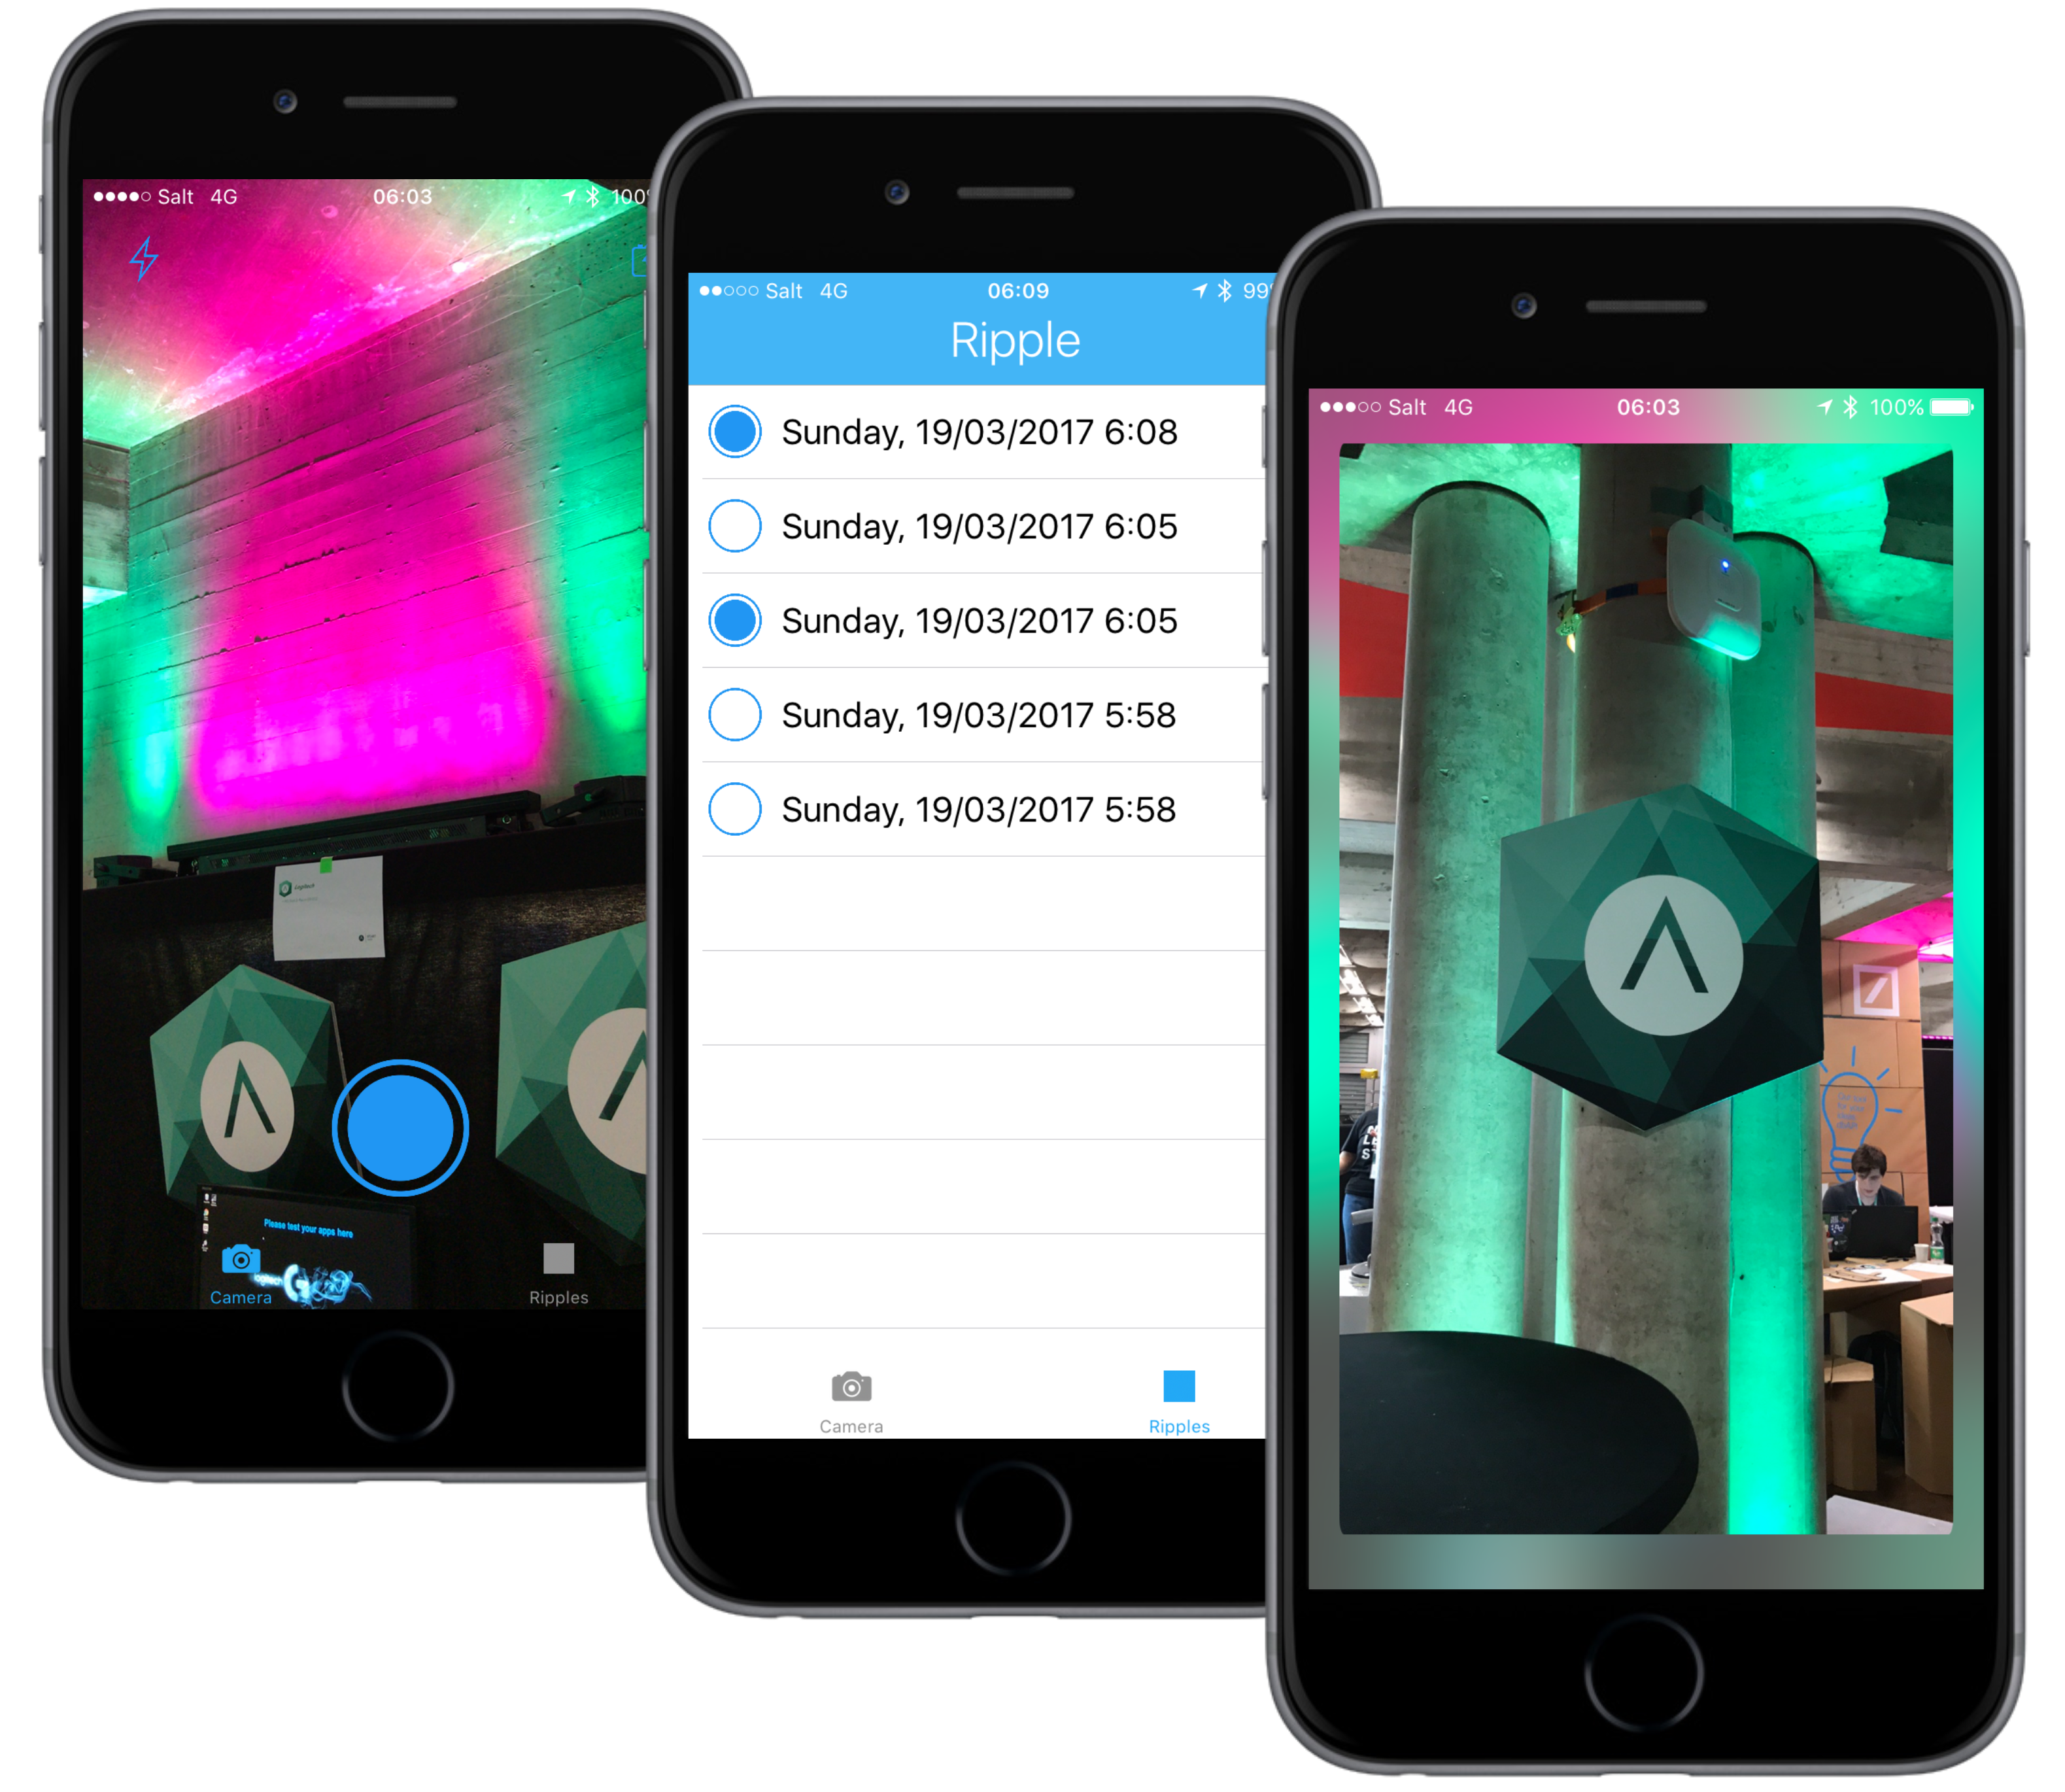
\includegraphics[width=\columnwidth]{rippleslide.png}
    \lfig{example}
    \vspace{-5mm} % use negative white space to fix too large gaps
	\caption{What our final product could look like. Includes a view to take photos (Left), a list of all received and opened photos (middle), and a screenshot of what a photo looks like right after when it's taken and before it's shared (right)}
\end{figure}



\section{Requirements}
Describe system setup, components, external libraries, hardware etc.

\subsection{Hardware}
Our proposed app is a social networking app, relying on no additional hardware.

\subsection{Software (libraries and frameworks)}
We plan on implementing our own P2P logic, as most existing solutions build P2P technology that heavily relies on web, and not bluetooth. In addition to that, our proposed architecture introduces a rather centralized element, \textit{the Tracker}, which has a vastly different role than a node, and as such, calls to a different underlying P2P technology. However, if suitable, we will try to implement

\subsection{3rd party services}
We will use bluetooth technology to transmit photos between the individual nodes. We also intend on using Amazon AWS EC2 to use as a tracker, allowing the individual nodes to ping for all photos that should be delivered, and for the senders to actually deliver them.

\begin{figure}[h]
	\centering
    \includegraphics[width=\columnwidth]{overview.jpg}
    \lfig{system-overview}
    \vspace{-5mm} % use negative white space to fix too large gaps
	\caption{System Overview~\cite{estimote}}
\end{figure}

\section{Work Packages}
Breakdown the work to subtasks to meet the project requirements.
Define and describe these tasks.

\begin{itemize}
        \item {\bf WP1}:  Build an Android front-end that can take pictures and temporally saves it in a local storage.  \ldots    
        \item {\bf WP2}:  Build an Android back-end which acts as a node. It should be able to transfer files from one device to another using bluetooth, and save it with the local storage.
        \item {\bf WP3}: Connect WP1 and WP2 such that all transmitted files are displayed on the receiver using the front-end.    
        \item {\bf WP4}: Initialize and configure backend server.    
        \item {\bf WP5}: Create all API endpoints which accept ID's, and checks which photos are delivered to which devices. The uuid can act as an unique identifier for each node.    
        \item {\bf WP6}: Implement logic in the node backend that pings other phones for a photo, if a photo was not yet received (which is determined by the received photo id's).   
         \item {\bf Optional WP7}: The final part would be to change the data-transmission through packages, instead of using a one-to-one connection, where only a single node communicates with another node.
\end{itemize}
 
\section{Milestones}


\subsection{Schedule}
We form a temporal schedule on what tasks should be achieved, sorted by upcoming dates.
\begin{enumerate}
\item  \textbf{24. Nov. 2017}: We plan on finishing the work packages that are considered part of the app, namely \textit{WP1} and \textit{WP2}, .
\item  \textbf{1. Dec. 2017}: We intend to finish setting up the central tracker, and all it's API functions. These are part of \textit{WP3} and \textit{WP4}.
\item \textbf{8. Dec. 2017}: We plan to do a naive implementation of the entire system, where the tracker communicates with the phones the photos to be downloaded, and the photos are communicated between the individual nodes. This is concluded by \textit{WP5} and  \textit{WP6} 'putting the components together'.
\item \textbf{15. Dec. 2017}: Assuming all went as planned, we would be able to implement some more efficient partial-data-delivery system as modern system like bittorent do. If this is not possible, however, we plan on using this time as a buffer, finishing any tasks from the previous weeks that are left undone. Assuming we have the time, we would continue with \textit{Optional WP7}.
\end{enumerate}


\subsection{Assignment to team members}

Luckily, all tasks are extensive enough that a majority of team members can work on the individual working package individually. As such, for each deadline (\textit{24. Nov. 2017}, \textit{1. Dec. 2017}, \textit{8. Dec. 2017}, \textit{15. Dec .2017}), we plan to split the team into two sub-sections, each of which handles one working package. Within each working package, we intend to have a flexible schedule amongst team-members, as this has proven to be effective in the past few Android projects.

\bibliographystyle{abbrv}
\bibliography{report}  % sigproc.bib is the name of the Bibliography in this case
% You must have a proper ".bib" file

%\balancecolumns % GM June 2007

\end{document}
